A roda omnidirecional aparece em vários modelos na literatura, como exemplo o design feito por J. Graboweicki em 1919 \cite{patent_US1305535A}
o design feito por Josef Blumrich em 1972 \cite{patent_US3789947A}.
A roda consiste em rolos perpendiculares (90°) a direção de giro da roda,o efeito é sua capacidade da roda se mover em mais de uma direção ao mesmo tempo.

\begin{figure}[h]
	\centering
	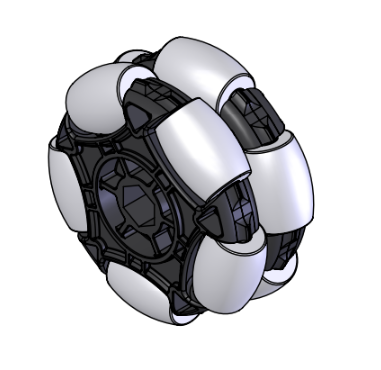
\includegraphics{figures/omniwheel}
	\caption{Modelo de uma Omniwheel \cite{draw_omniwheel}}
\end{figure}

Uma variação da roda omnidirecional é a roda mecanum, inventada por Bengt Ilon \cite{patent_US3876255A}, que possue rolos em 45°.